\chapter{Precomputed Radiance Transfer}\label{chp:prt}
In every frame, the rendering equation computes the light transfer, the process of the lights are transferred from the light sources through the surfaces of the objects in the scene into the camera. If the scene is static, this computation should be the same, and we can precompute them in advance to reach high performance.

The main insight of precomputed radiance transfer (PRT)\cite{a:PrecomputedRadianceTransferforRealTimeRenderinginDynamicLowFrequencyLightingEnvironments} is that the integral can be split into a precomputed transfer function that includes the effects of self-shadowing and inter-reflections, and a runtime computation that efficiently combines the transfer function with the dynamically changing environment map.

To achieve this goal, PRT projects the lighting onto a set of basis functions, such as spherical harmonics (SH), over the sphere. Then we can substituting the SH lighting coefficient to the rendering equation to compute the transfer function, represented as a vector or matrix. At runtime, the outgoing radiance is then just the dot product of these two coefficients of the basis functions. See section \ref{sec:prt}.

In this chapter, we first review some properties of the basis functions. Then we'll discuss PRT and how to precompute these transfer function (vector or matrix). First we introduce PRT for low-frequency, then for all-frequency lighting environment.


\section{Basis Functions}
In mathematics, a \textit{basis function} is an element of a particular basis for a \textit{function space}. Every continuous function in the function space can be represented as a linear combination of basis functions, just as every vector in a vector space can be represented as a linear combination of basis vectors. For example, the collection of quadratic polynomials with real coefficients has $\{1,t,t^{2}\}$ as a basis. Every quadratic polynomial can be written as $a1+bt+ct^{2}$, that is, as a linear combination of the basis functions $1, t$, and $t^{2}$.

\begin{figure}\label{f:projection-and-reconstruction}
	\begin{center}
		\begin{subfigure}[b]{0.49\textwidth}
			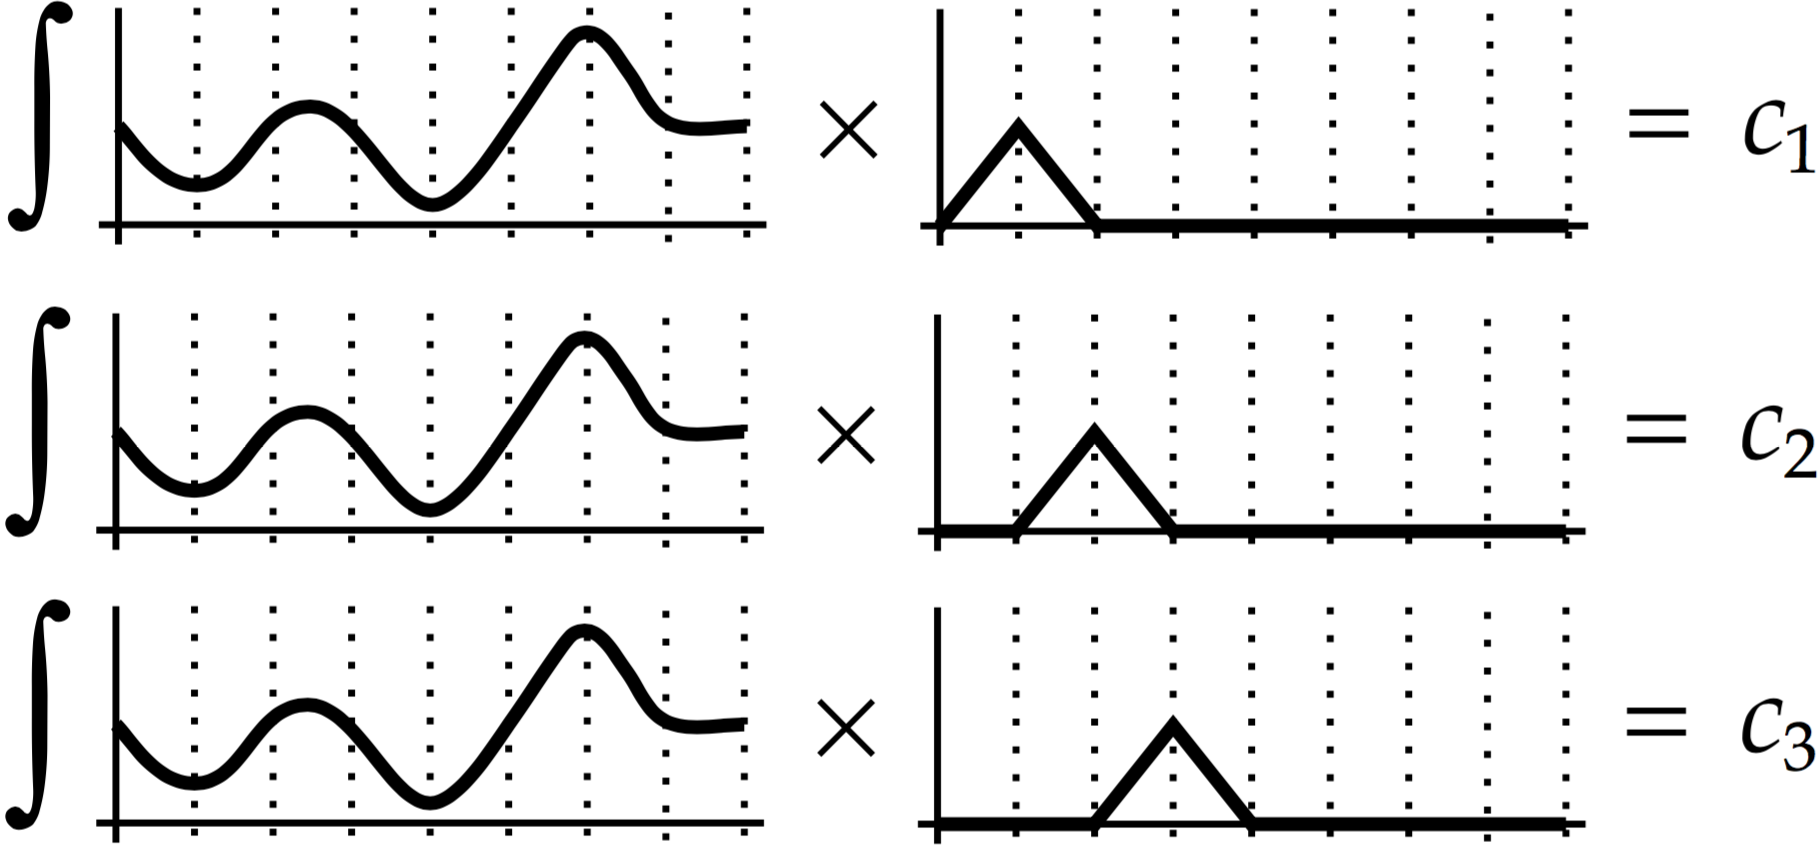
\includegraphics[width=0.95\textwidth]{graphics/prt/prt-1}
			\caption{Projection}
		\end{subfigure}
		\begin{subfigure}[b]{0.49\textwidth}
			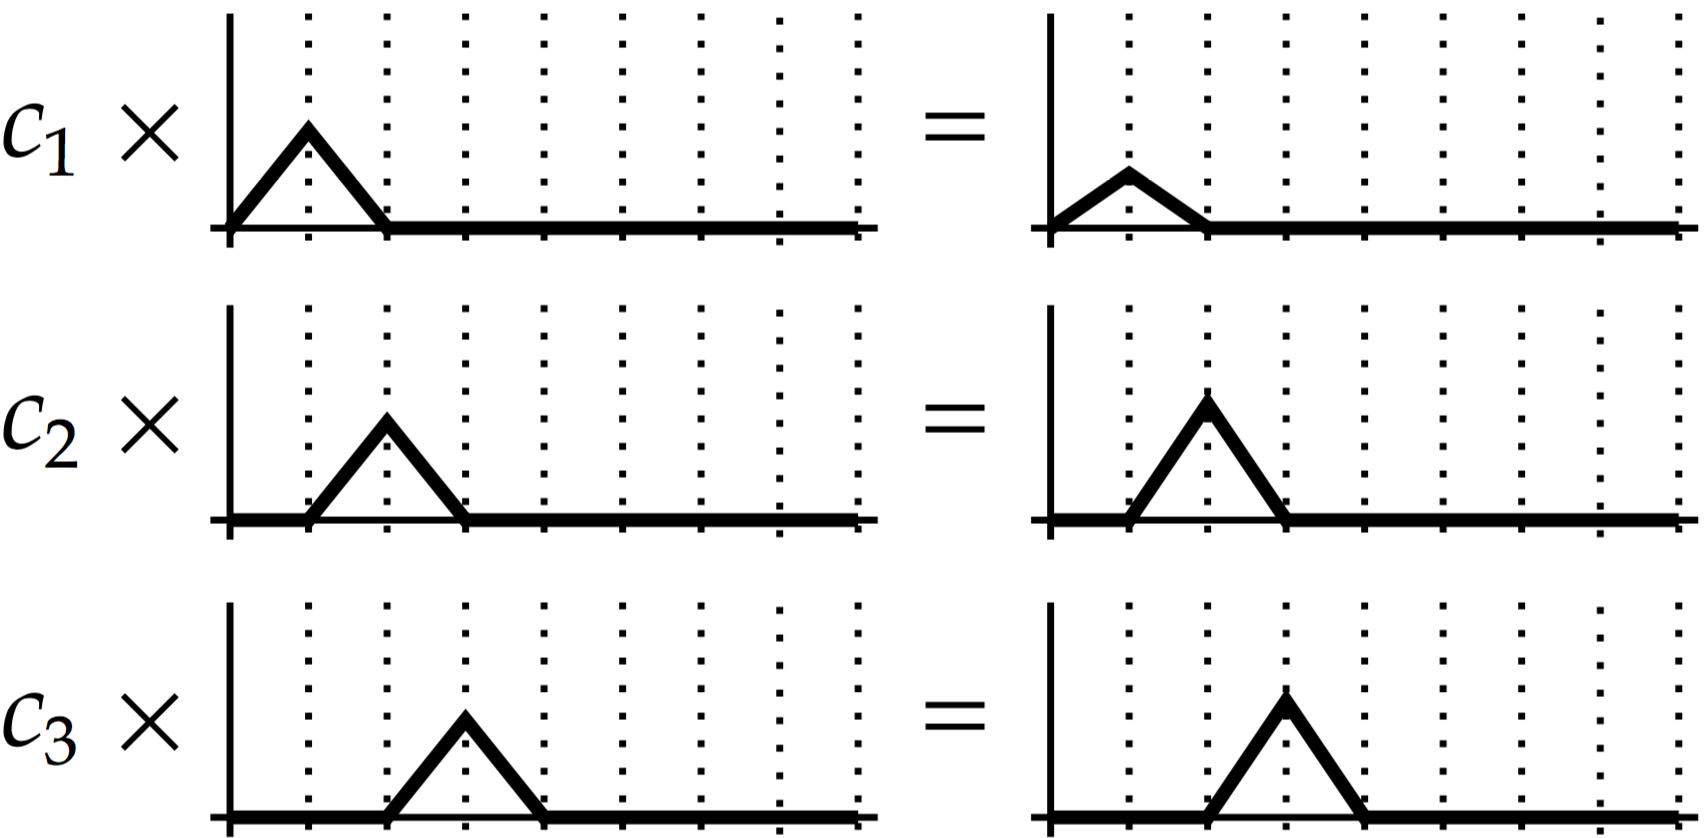
\includegraphics[width=0.9\textwidth]{graphics/prt/prt-2}
			\caption{Reconstruction}
		\end{subfigure}
	\end{center}
	\caption{Basis functions are small pieces of signal that can be scaled and combined to produce an approximation to an original function, and the process of working out how much of each basis function to sum is called projection.}
\end{figure}

So if we've known the basis functions, we can use a vector (the coefficients) to represent a function. Given some function $f(t)$ defined over $T$ and the basis functions $B_i(t)$, the function can be \textit{projected} (see figure \ref{f:projection-and-reconstruction}(a)) into its coefficients vis the integral:

\begin{equation*}
	c_i=\int f(t)B_i(t)dt=:\langle f(t),B_i(t)\rangle
\end{equation*}

\textit{Reconstruction}, is done by scaling the basis functions with the coefficients $c_i$, see figure \ref{f:projection-and-reconstruction}(b), and then summing them up:

\begin{equation*}
	f(t)\approx\tilde{f}(t) =\sum_{i}^{N}c_iB_i(t)=\raisebox{-.5\height}{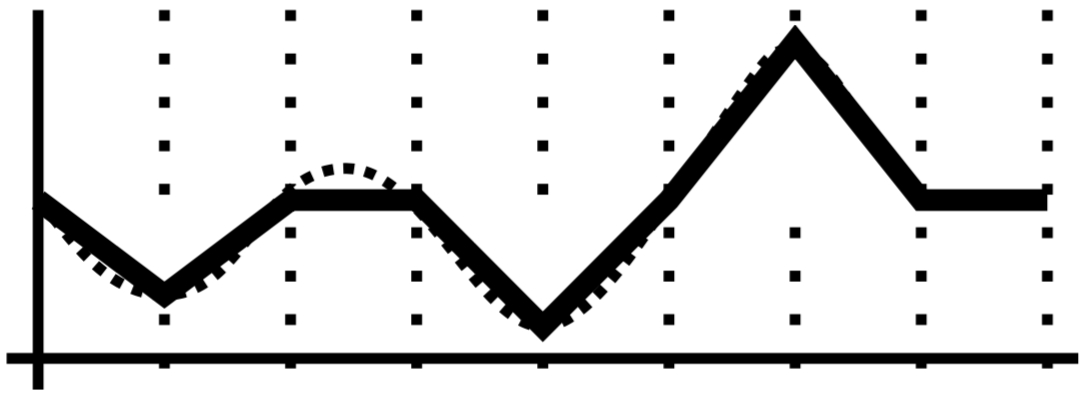
\includegraphics[width=0.25\textwidth]{graphics/prt/prt-3}}
\end{equation*}

where $N$ is the number of the coefficients. If $N$ is less than the number of the basis functions, the result is an approximation of the original function, denoted by $\tilde{f}(t)$.

In the above example we have used a set of linear basis functions, giving us a piecewise linear approximation to the input function. There are many basis functions we can use, but some of the most interesting are grouped into a family of functions called \textit{orthogonal polynomials}.

Orthogonal polynomials are sets of polynomials that have an intriguing property -- when you integrate the product of any two of them, if they are the same you get a constant value and if they are different you get zero:

\begin{equation*}
	\int_{-1}^{1}F_m(x)F_n(x)dx=\begin{cases}
		0 & \text{ for } n\neq m\\
		1 & \text{ for } n=m
	\end{cases}
\end{equation*}

We can also specify the more rigorous rule that integrating the product of two of these polynomials must return $0$ or $1$, and this sub-family of functions are known as the \textit{orthonormal basis functions}. Intuitively, it's a like the functions do not "overlap" each other's influence while still occupying the same space, the same effect that allows the Fourier transform to break a signal into it's component sine waves.



\subsection{Legendre Polynomials}
The one family we are most interested in are called the Legendre polynomials\footnote{\url{https://en.wikipedia.org/wiki/Legendre_polynomials}}, specifically the \textit{Associated Legendre Polynomials}. Traditionally represented by the symbol $P$, the associated Legendre polynomials have two arguments $l$ and $m$, are defined over the range $[-1,1]$ and return real numbers (as opposed to the ordinary Legendre Polynomials which return complex values).

According to Wolfram\footnote{\url{http://mathworld.wolfram.com/AssociatedLegendrePolynomial.html}}, the associated Legendre polynomials $P^{m}_{l}(x)$ and $P^{-m}_{l}(x)$ generalize the Legendre polynomials $P_l(x)$ and are solutions to the associated Legendre differential equation, where $l$ is a positive integer and $m=0,\cdots,l$. For positive $m$, they can be given in terms of the unassociated polynomials by:

\begin{equation*}
\begin{aligned}
	p^{m}_{l}(x)&=(-1)^{m}(1-x^{2})^{m/2}\frac{d^{m}}{dx^{m}}P_l(x)\\
	&=\frac{(-1)^{m}}{2^{l}l!}(1-x^{2})^{m/2}\frac{d^{l+m}}{dx^{l+m}}(x^{2}-1)^{l}
\end{aligned}
\end{equation*}

where $P_l(x)$ are the unassociated Legendre polynomials. The associated Legendre polynomials for negative $m$ are then defined by:

\begin{equation*}
	P_{l}^{-m}=(-1)^{m}\frac{(l-m)!}{(l+m)!}P^{m}_{l}(x)
\end{equation*}

\begin{figure}
\sidecaption
	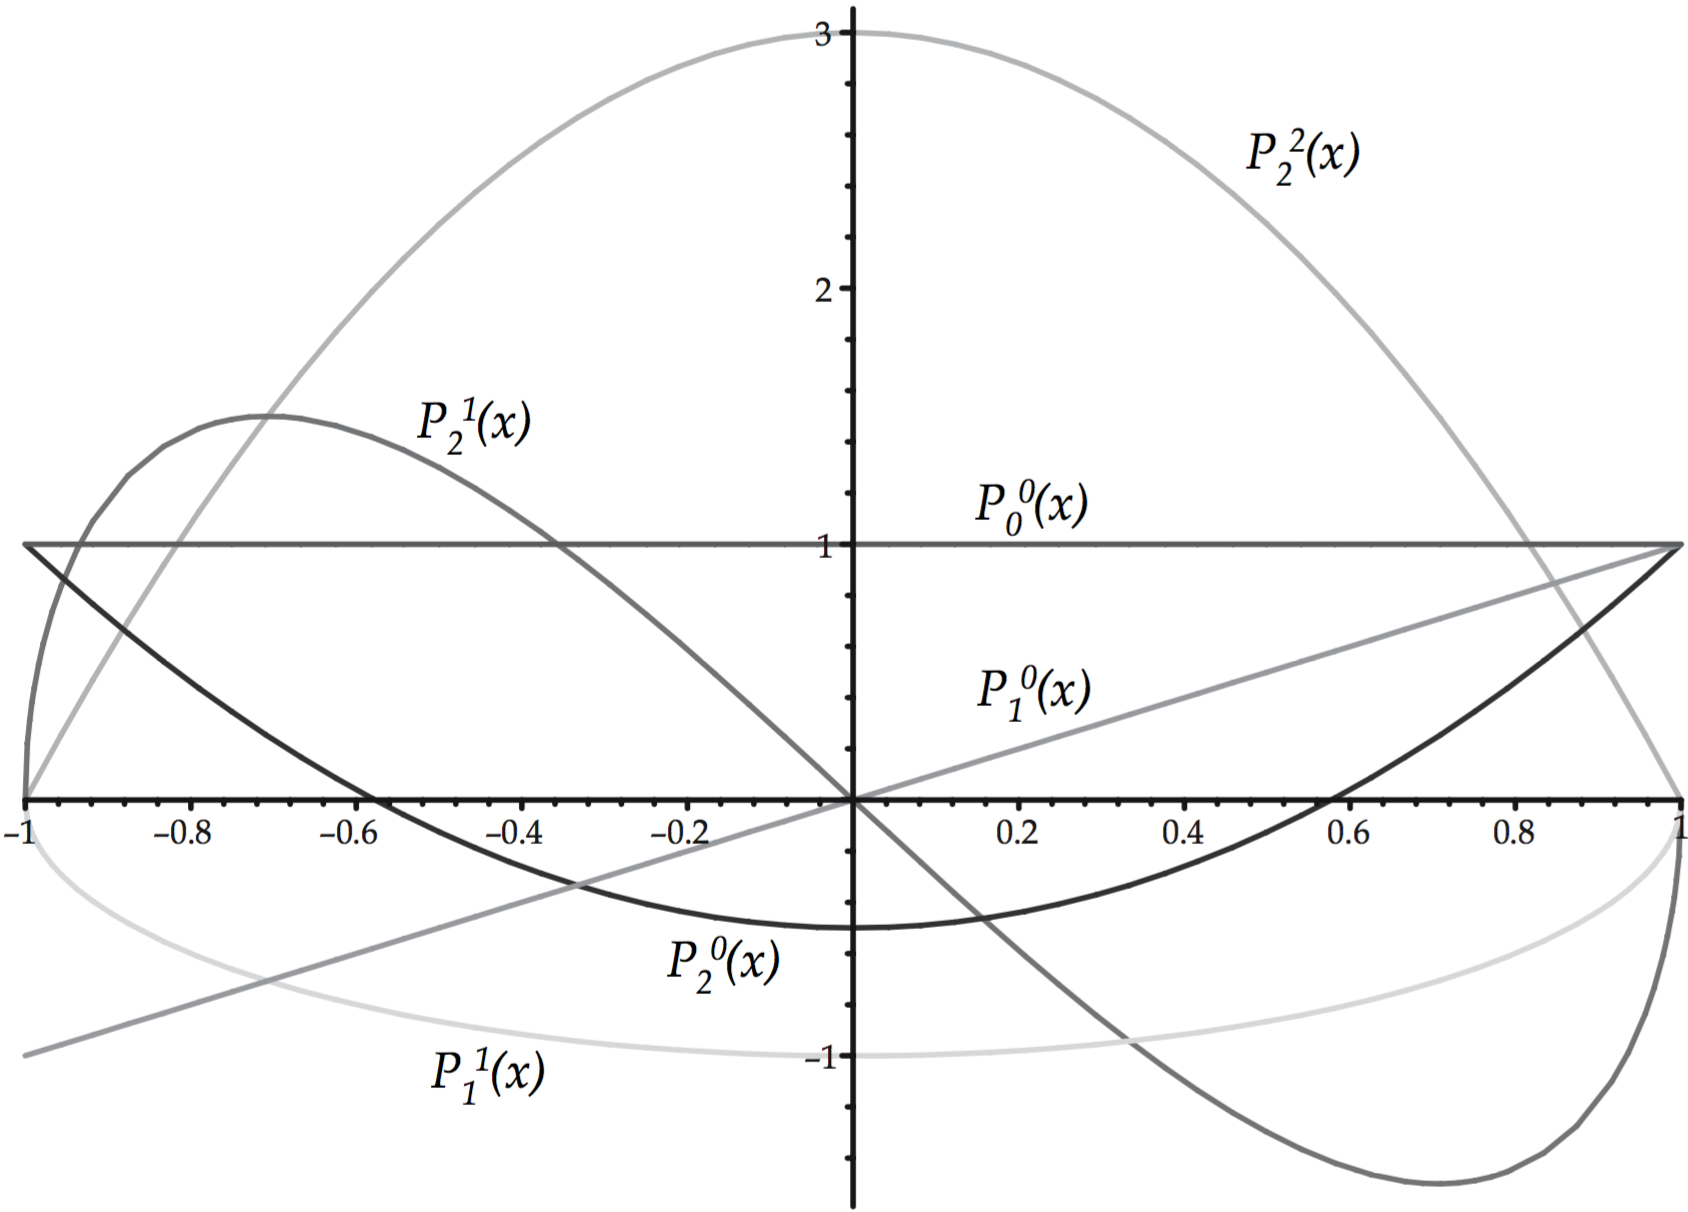
\includegraphics[width=0.65\textwidth]{graphics/prt/prt-5}
	\caption{The first six associated Legendre polynomials.}
\end{figure}

The two arguments $l$ and $m$ break the family of polynomials into \textit{bands} of functions where the argument $l$ is the \textit{band index}. Inside a band the polynomials are orthogonal with regard to a constant term and between bands they are orthogonal with different constant.



\subsection{Spherical Harmonics}
Spherical harmonics (SH)\footnote{The SH functions in general are defined on imaginary numbers but we are only interested in approximating real functions over the sphere.} are a series of special function defined on the surface of a sphere used to solve some kinds of differential equations. As Fourier series are a series of functions used to represent functions on a circle, spherical harmonics are a series of functions that are used to represent functions defined on the surface of a sphere.

The associated Legendre polynomials are at the heart of the spherical harmonics. Given the standard parameterization of points on the surface of a unit sphere into spherical coordinates:

\begin{equation*}
	(sin\theta cos\varphi,sin\theta sin\varphi,cos\theta)\to(x,y,z)
\end{equation*}

the SH function is traditionally represented by the symbol $y$:

\begin{equation*}
	y^{m}_{l}(\theta,\varphi)=\begin{cases}
		\sqrt{2}K^{m}_{l}cos(m\varphi)P^{m}_{l}(cos\theta), &m>0\\
		\sqrt{2}K^{m}_{l}sin(-m\varphi)P^{-m}_{l}(cos\theta), &m<0\\
		K^{0}_{l}P^{0}_{l}(cos\theta), & m=0
	\end{cases}
\end{equation*}

where $P$ is the same associated Legendre polynomials we look at earlier and $K$ is just a scaling factor to normalize the functions:

\begin{equation*}
	K^{m}_{l}=\sqrt{\frac{(2l+1)}{4\pi}\frac{(l-|m|)!}{(l+|m|)!}}
\end{equation*}

In order to generate all the SH functions, the parameters $l$ and $m$ are defined slightly differently from the Legendre polynomials -- $l$ is still a positive integer starting from $0$, but $m$ takes signed integer values from $-l$ to $l$.

Sometimes it is useful to think of the SH functions occurring in a specific order so that we can flatten them into a 1D vector, so we will also define the sequence $y_i$:

\begin{equation*}
	y^{m}_{l}(\theta,\varphi)=y_i(\theta,\varphi) \text{\quad\quad  where\quad} i=l(l+1)+m
\end{equation*}

The functions actually look like when plotted as spherical functions can be see in figure \ref{f:sperical-harmonic}.

\begin{figure}
\sidecaption
	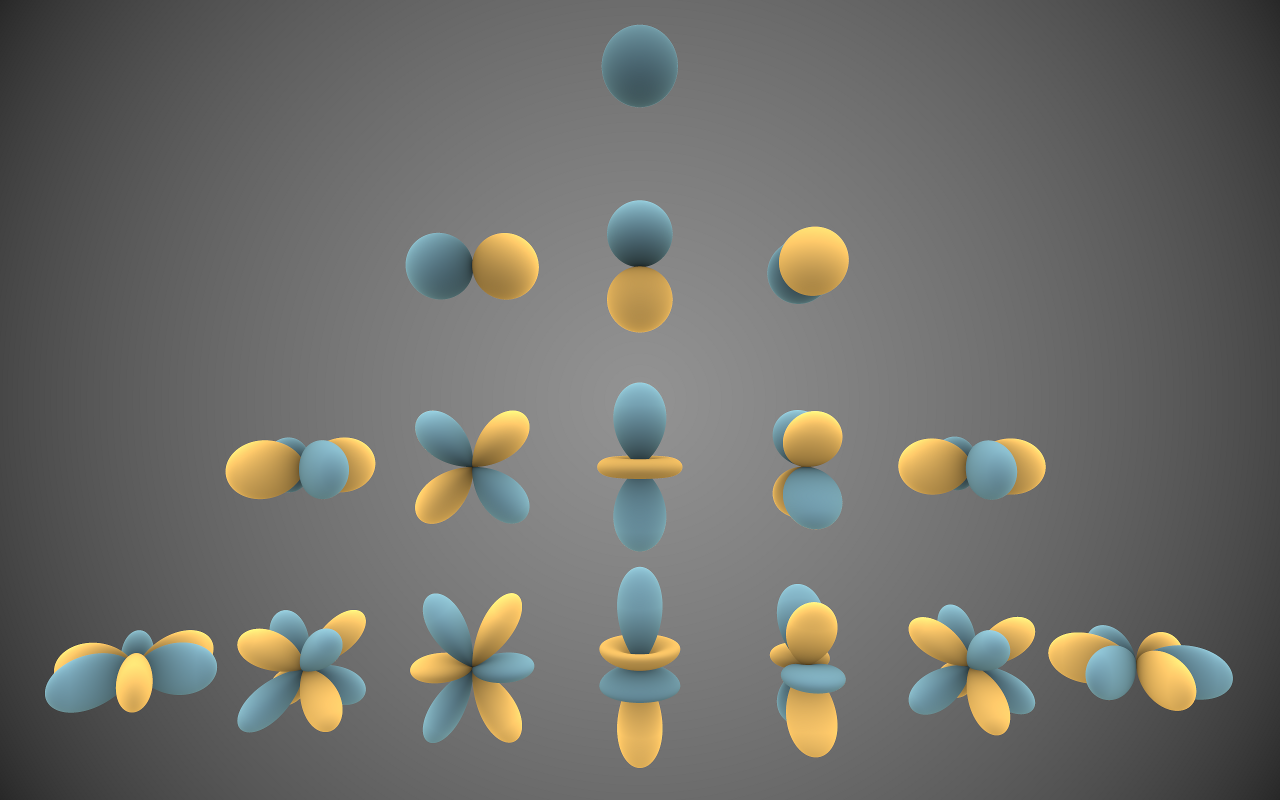
\includegraphics[width=0.65\textwidth]{graphics/prt/prt-4}
	\caption{Visual representations of the first 4 bands of real spherical harmonic functions. Blue portions are regions where the function is positive, and yellow portions represent regions where it is negative.}
	\label{f:sperical-harmonic}
\end{figure}



\subsubsection{SH Projection}
The process for projecting a spherical function into SH coefficients is very simple and the same as the basis functions. TO calculate a single coefficient for a specific band you just integrate the product of your function $f$ and the SH function $y$, in effect working out how much your function is like the basis function:

\begin{equation*}
	c_{l}^{m}=\int_{S}f(s)y^{m}_{l}(s)ds
\end{equation*}

To reconstruct the approximated function (notated by $f$ capped with a tilde), we just take the reverse process and sum scaled copies of the corresponding SH functions:

\begin{equation*}
	\tilde{f}(s)=\sum^{n-1}_{l=0}\sum^{l}_{m=-1}c^{m}_{l}y^{m}_{l}(s)=\sum^{n^{2}}_{i=0}c_iy_i(s)
\end{equation*}

Now you can see why an $n-$th order approximation will require $n^{2}$ coefficients. It can be proven that the true function $f$ could be reconstructed if we summed the infinite series of all SH coefficients, so every reconstruction we will make will be an approximation to the true function, technically known as a \textit{band-limited} approximation where band-limiting is just the process of breaking a signal into it's component frequencies and removing frequencies higher than some threshold.

\begin{figure*}
	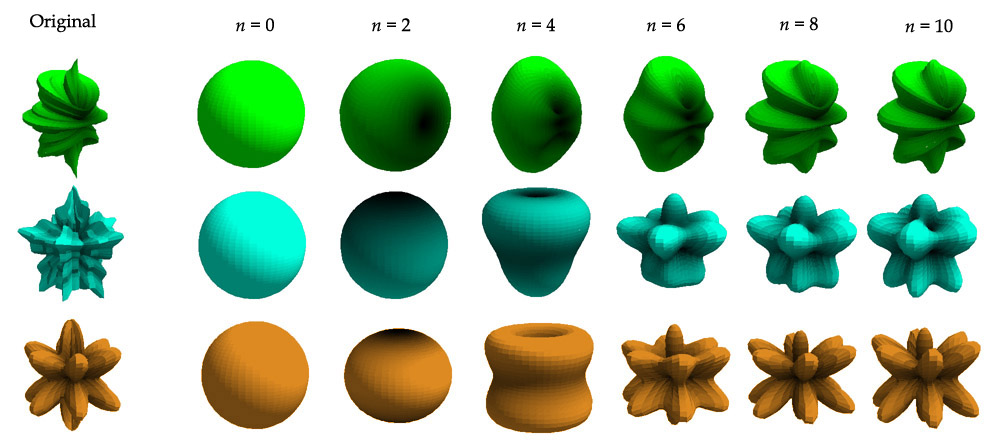
\includegraphics{graphics/prt/prt-6-2}
	\caption{SH projection of functions with increasing orders of approximation.}
\end{figure*}

So if there is a low-frequency function, we can use only few coefficients to represent the function using SH.



\subsubsection{Properties of SH Functions}
The SH functions have a bunch of interesting properties that make them more desirable for our purposes than other basis functions.

\paragraph{Basic Properties} Firstly, the SH functions are not just orthogonal but orthonormal, meaning if we integrate $y_iy_j$ for any pair of $i$ and $j$, the calculation will return $1$ if $i=j$ and $0$ if $i\neq j$.


The SH functions are also \textit{rotationally invariant}. That is, given $g(s)=f(Q(s))$ where $Q$ is an arbitrary rotation over $S$ then:

\begin{equation*}
	\tilde{g}(s)=\tilde{f}(Q(s))
\end{equation*}

This is analogous to the shift-invariance property of the Fourier transform. Practically, this property means that SH projection causes no aliasing artifacts when samples from $f$ are collected at a rotated set of sample points.

Orthonormality of the SH basis provides the useful property that given any two functions $a$ and $b$ over $S$, their projections satisfy:

\begin{equation*}
	\int \tilde{a}(s)\tilde{b}(s)ds=\sum^{n^{2}}_{i=1}a_ib_i
\end{equation*}

In other words, integration of the product of bandlimited functions reduces to a dot product of their projection coefficients. This property is very useful in the rendering equation, we can project both incoming light and the transfer function into SH coefficients then orthogonality guarantees that the integral of the function's products is the same as the dot product of their coefficients.


\paragraph{Product Projection} Projection of the product of a pair of spherical functions $c(s)=a(s)b(s)$ where $a$ is known and $b$ unknown can be viewed as a linear transformation of the projection coefficients $b_j$ via a matrix $\mathbf{M}$ (Say we have some arbitrary spherical light source function $b(s)$ that we don't know yet. We also have some shadowing function for a particular point on the surface $a(s)$ that describes how light at that point is shadowed, and we can evaluate it using a ray tracer):

\begin{equation*}
\begin{aligned}
	c_i=&\int a(s)(b_jy_j(s))y_i(s)ds\\
	   =&(\int a(s)y_i(s)y_j(s)ds)b_j=(a_k\int y_i(s)y_j(s)y_k(s)ds)b_j\\
	   =&\mathbf{M}_{ij}b_j
\end{aligned}
\end{equation*}

The components of $\mathbf{M}$, a transfer matrix that we can use to transform from a light source into a shadowed light source using a simple matrix-vector multiply, can be computed by integrating the \textit{triple product} of basis functions using recurrences derived from the well known Clebsch-Gordan series. It can also be computed using numerical integration without SH-projecting the function $a$ beforehand.

This property is the core idea of PRT which we will see in section \ref{sec:prt}. In PRT, we precompute a transfer matrix for glossy surface point and a vector for a diffuse surface.  



\paragraph{Convolution}
We denote convolution of a circularly symmetric kernel function $h(z)$ with a function $f$ as $h*f$. Note that $h$ must be circularly symmetric (and hence can be defined as a simple function of $z$ rather than $s$) in order for the result to be defined on $\mathbf{S}$ rather than the higher-dimensional rotation group $\mathbf{SO}(3)$. Projection of the convolution satisfies:

\begin{equation*}
	(h*f)^{m}_{l}=\sqrt{\frac{4\pi}{2l+1}}h^{0}_{l}f^{m}_{l}=a^{0}_{l}h^{0}_{l}f^{m}_{l}
\end{equation*} 

In other words, the coefficients of the projected convolution are simply scaled products of the separately projected functions. Note that because $h$ is circularly symmetric about $z$, its projection coefficients are nonzero only for $m=0$. The convolution properties provides a fast way to convolve an environment map with a hemispherical cosine kernel, defined as $h(z) = max(z,0)$, to get an irradiance map, for which the $h_l^{0}$ are given by an analytic formula. The convolution property can also be used to produce prefiltered environment maps with narrower kernels.





\section{Diffuse PRT}\label{sec:prt}
Suppose the scene is static, the main idea of PRT is to precompute the radiance transfer for every point (vertex or pixel according to the implementation).

In the original paper of PRT\cite{a:PrecomputedRadianceTransferforRealTimeRenderinginDynamicLowFrequencyLightingEnvironments}, the light source is represented using SH functions, and the inter-reflections and shadows of the surface are treated as a transfer vector or matrix, then the result is the product of the vector (or matrix) and the coefficients of the light source, by the property of SH (product projection).

So another assumption of PRT is low-frequency of the light source (usually environment maps), because we should use few coefficients to represent the light source so the pre-computed data, the vectors or matrices, are smaller to save memory and reduce runtime dot product computation. In such case, only very soft shadows can be handled.

Nevertheless, some other approaches have been proposed to represent all-frequency lighting. In this section, we'll discuss the basis of PRT, and we'll talk about all-frequency lighting in the next section.



\subsection{Basis}
For simplicity, we'll start with diffuse surfaces, because it's reflected light is view-independent and we only need a vector to represent the transfer function of a point. To derive PRT for the diffuse case we are going to start with the direct term from the Neumann expansion of the rendering equation:

\begin{equation*}
\begin{aligned}
	L(p\to\vec{d})=&L_0(p\to\vec{d})+L_1(p\to\vec{d})+\cdots \\
	L_0(p\to\vec{d})=&\int_\Omega f_r(p,\vec{s}\to\vec{d})L_{env}(\vec{s})V(p\to\vec{s})H_{N_p}(-\vec{s})d\vec{s}
\end{aligned}
\end{equation*}

and make several simplifying assumptions: For diffuse objects light is reflected equally in all directions, so outgoing radiance is independent of view direction; This also means the BRDF is just a constant (and independent of direction) so it can be pulled out of the integral. So the direct term can be rewritten as following:

\begin{equation*}
	L_0(p)=\frac{\rho_d}{\pi}\int L_{env}(\vec{s})V(p\to\vec{s})H_{N_p}(-\vec{s})d\vec{s}
\end{equation*} 

where $\rho_d$ represents the diffuse reflectivity of the surface, and is a number between $0$ and $1$. The divide by $\pi$ enforces energy conservation. We also assume the source radiance function is at infinity, this means we only need to concern ourselves with the direction $s$.

\begin{figure}\label{f:prt-1}
	\begin{center}
		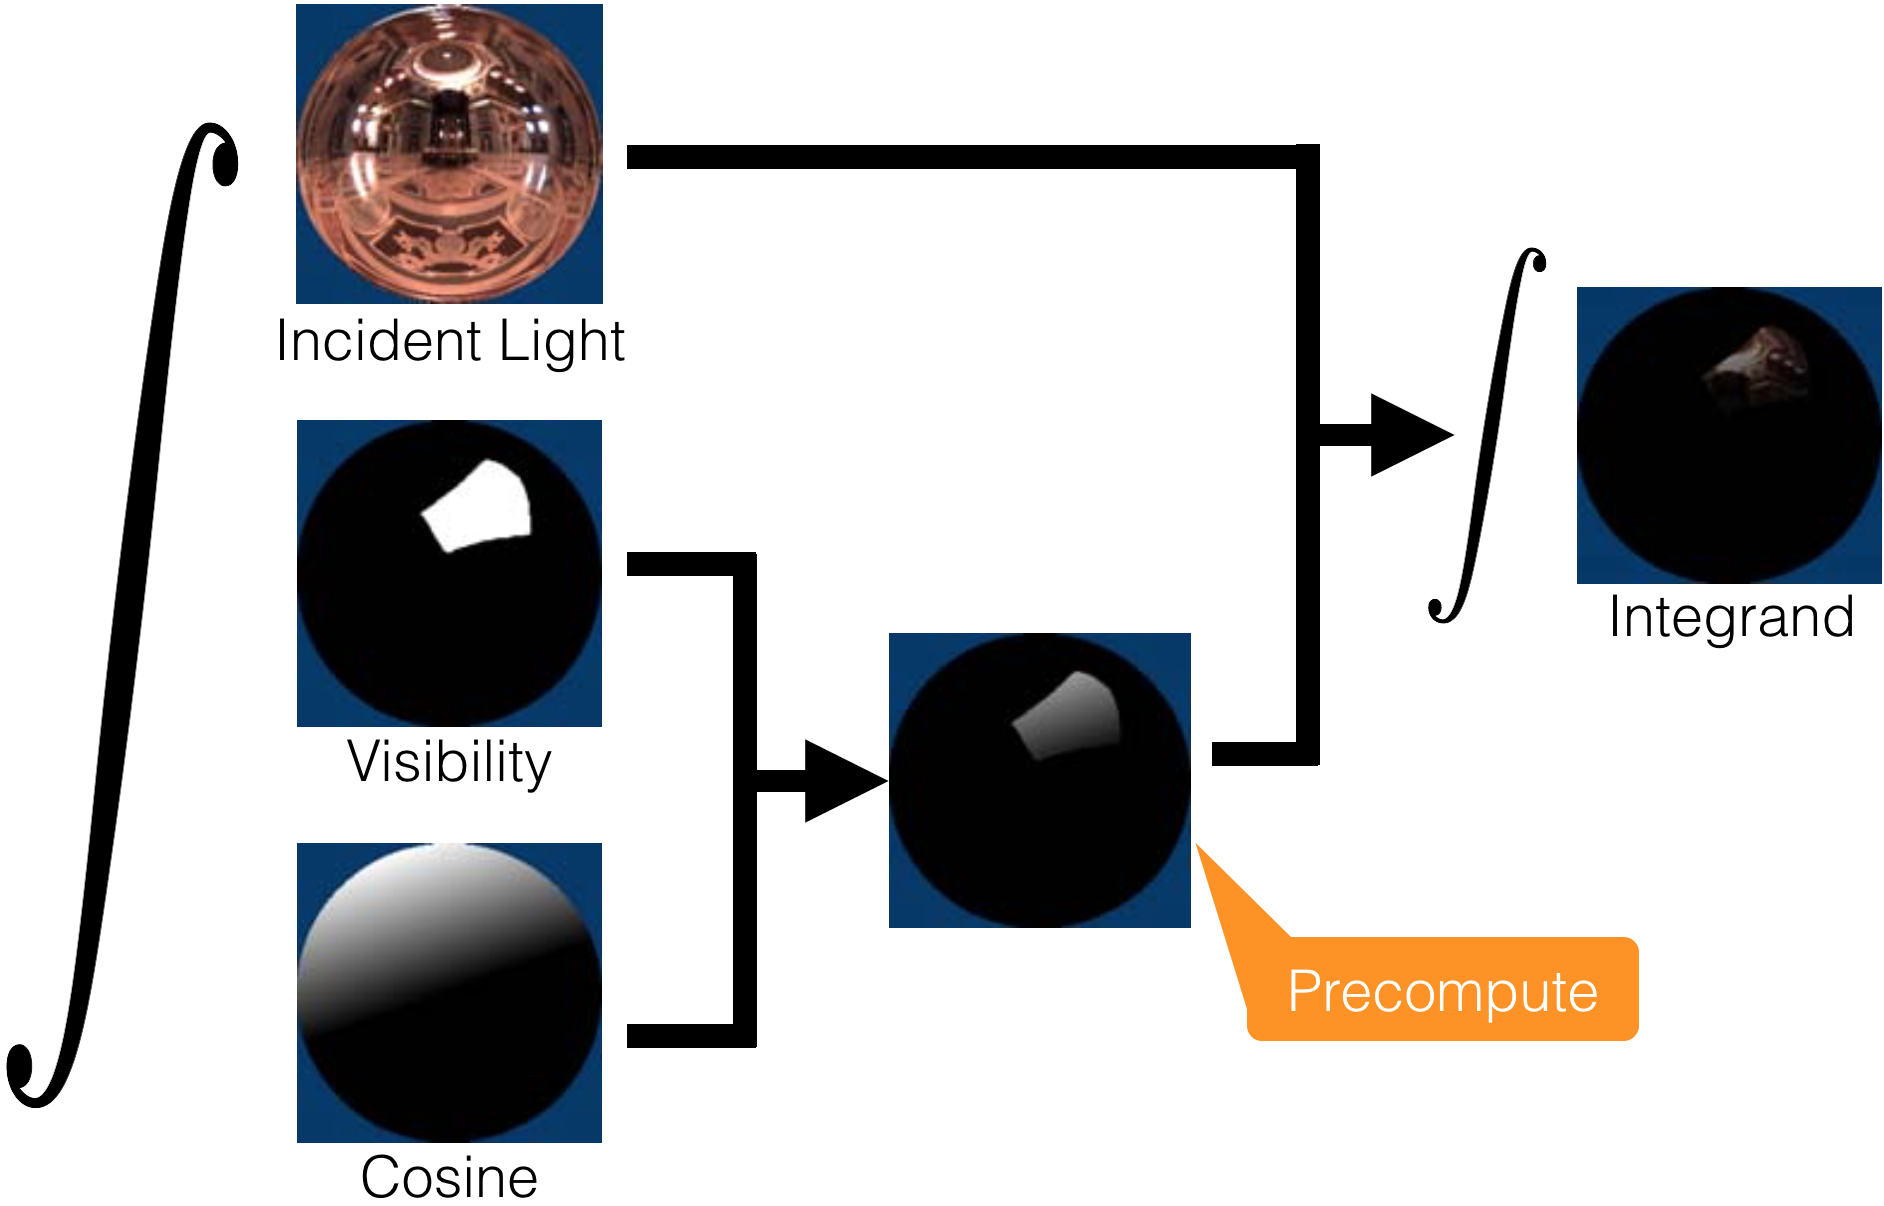
\includegraphics[width=0.85\textwidth]{graphics/prt/prt-7}
	\end{center}
	\caption{The main tricky we are going to use for precomputed radiance transfer is to combine the visibility and the cosine into one function.}
\end{figure}

Visually, we integrate the product of three functions (light, visibility, and cosine). The main tricky we are going to use for precomputed radiance transfer is to combine the visibility and the cosine into one function (cosine-weighted visibility or transfer function), see figure \ref{f:prt-1}, which we integrate against the lighting.



\subsection{Approximating the Light Source}
The light source $L_{env}$ can be seen as an unknown function, and the combined cosine-weighted visibility or transfer function the known. According to the property of SH, we can use SH coefficients represent the light source, and the transfer function becomes a transfer vector (or matrix) which can be precomputed. 
 
Now we are going to approximate the source radiance function with its projection into a set of basis functions on the sphere:

\begin{equation*}
	L_{env}(\vec{s})\approx\sum_{i}l_iy_i(\vec{s})
\end{equation*}

where $l_i$ are the projection coefficients of a particular lighting environment. 



\subsection{Transfer Vector}
We can plug this approximation directly into the reflected radiance equation. Since it's linear, sum of integrals = integral of sums, we can move sum outside integral. Everything within the integral can be precomputed (since it is independent of the actual lighting environment being used):

\begin{equation*}
	L_0(p)=\frac{\rho_d}{\pi}\sum_i l_i\int_{\Omega}y_i(\vec{s})V(p\to\vec{s})H_{N_p}(-\vec{s})d\vec{s}
\end{equation*}

The integral represents a transfer coefficient -- it maps how direct lighting in basis function l becomes outgoing radiance at point p. The set of transfer coefficients is a transfer vector that maps lighting into outgoing radiance:

\begin{equation*}
	L_0(p)=\frac{\rho_d}{\pi}\sum_i l_i t^{0}_{pi}
\end{equation*}

We can fold the diffuse reflectivity into the transfer vector as well:

\begin{equation*}
	L_0(p)=\sum_i l_i t^{0}_{pi}
\end{equation*} 

A similar process can be used to model the other bounces, so that a final vector can be computed and used to map source radiance to outgoing radiance at every point on the object.

\begin{equation*}
	\begin{aligned}
		L(p)=&\sum_i l_i(t^{0}_{pi}+t^{1}_{pi}+\cdots)\\
		    =&\sum_i l_i t_{pi}
	\end{aligned}
\end{equation*}



\subsection{Rendering}
Outgoing radiance is then just the dot product of the lights projection coefficients with the transfer vector.

\begin{equation*}
	L(p)=\sum^{n}_{i}l_it_{p,i}
\end{equation*}

At run-time, we need to lookup the transfer vector at every pixel. A (vertex/pixel)-shader then computes the dot-product between the coefficient vectors. The result of this computation is the outgoing radiance at that point.




\subsection{Precomputation}
The main question is how to evaluate the integral. We will evaluate it numerically using Monte-Carlo integration. This basically means, that we generate a random (and uniform) set of directions $s_j$, which we use to sample the integrand. All the contributions are then summed up and weighted by $4\pi/(\#samples)$.

The visibility $V(p\to \vec{s})$ needs to be computed at every point. The easiest way to do this, is to use ray-tracing.




\section{General PRT}
A transfer vector $(T_p)_i$ is useful for diffuse surfaces and represents a linear transformation on the lighting vector producing scalar exit radiance. In other words, each component of $(T_p)_i$ represents the linear influence that a lighting basis function $l_i$ on shading at $p$.

In this section, we'll derive general case for glossy (view-dependent) reflection. As the previous section, we'll be looking at an object sitting in free space, distant from the lighting environment that illuminates it. "Distant" means that location on the object does not affect the directional distribution of incident light. In other words, in absence of occlusion, the direct light incident upon all points on the object is the same, i.e., $L_{env}(p,\omega)=L_{env}(\omega)$ for all $p$.

As described in the earlier section, the environment map that we use for lighting the object is projected into a function basis $\{y_i\}$ with $i=1,\cdots,n$. This yields an approximation to the original environment map, and the approximation is fully defined by the vector $l$ of coefficients:

\begin{equation*}
	L_{env}(\omega)\approx\sum^{n}_{i=1}l_iy_i(\omega)
\end{equation*} 




\subsection{Goals -- What does $p$ look like, given $L_{env}$?}
We have two goals in this section:

\begin{enumerate}
	\item Global illumination with glossy reflections and time-varying lighting. Shiny BRDFs mean that the appearance of a point changes depending on where it is looked at from.
	\item We also want to approximate the lighting in \textit{free space} around the object. For example, if we can compute the lighting incident to points in free space in the landscape, we can shade moving objects (vehicles, characters, etc.) with lighting that is affected by the environment, and thus get color bleeding and soft shadowing effects onto the moving objects.
\end{enumerate}

\begin{figure}
\sidecaption
	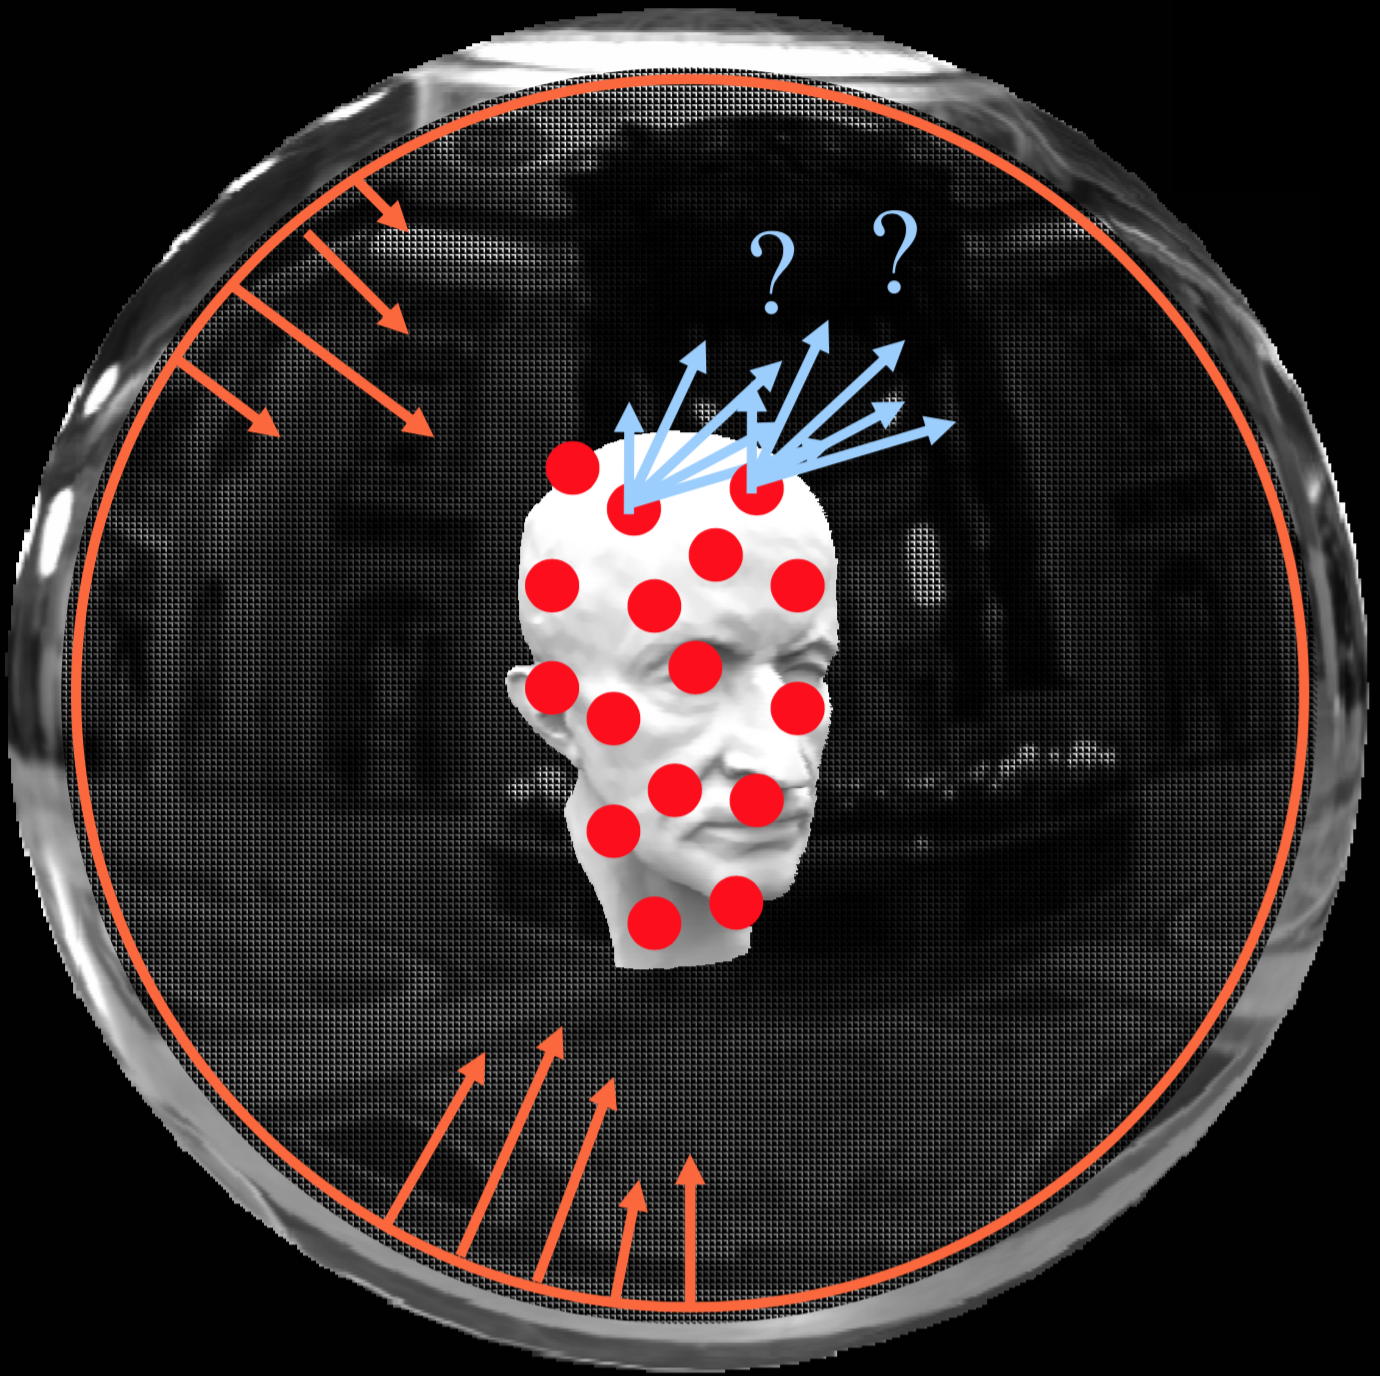
\includegraphics[width=0.65\textwidth]{graphics/prt/prt-8-1}
	\caption{Compute transfer matrices for many points and interpolate to get appearance of whole object.}
	\label{f:prt-goal-1}
\end{figure}

So what we want to know is: given some projected environment map, what do points on the object look like? That is, what is the directional distribution of outgoing light from each point? See figure \ref{f:prt-goal-1}. If we know these values, we can directly assign to pixels in an image.

The appearance of each point is linearly related to the distant lighting environment, so we are looking for some linear operator that takes as input the lighting environment, and produces the appearance of the point as output. In the end, we will represent this appearance in some linear basis, so the linear mapping will be, for each point, a matrix that maps the coefficients of incident, distant lighting environment into coefficients for outgoing radiance for the point $p$:

\begin{equation*}
	L_{env}(\omega)\to L_{out}(p\to\omega)
\end{equation*}

We'll compute this mapping for many points on the object, so that we can get a reasonable approximation for the appearance of the whole object by interpolating from these samples. See figure \ref{f:prt-goal-1}.

The other question is: what do the points near but not on the object "see" when the object is illuminated using an environment map? In other words, how does the presence of the object affect the lighting that impinges upon these points in free space?

Let's concentrate on a single point $p$ somewhere near the object, see figure \ref{f:prt-goal-2}. What does the point $p$ see can be decided by the following:

\begin{figure}
\sidecaption
	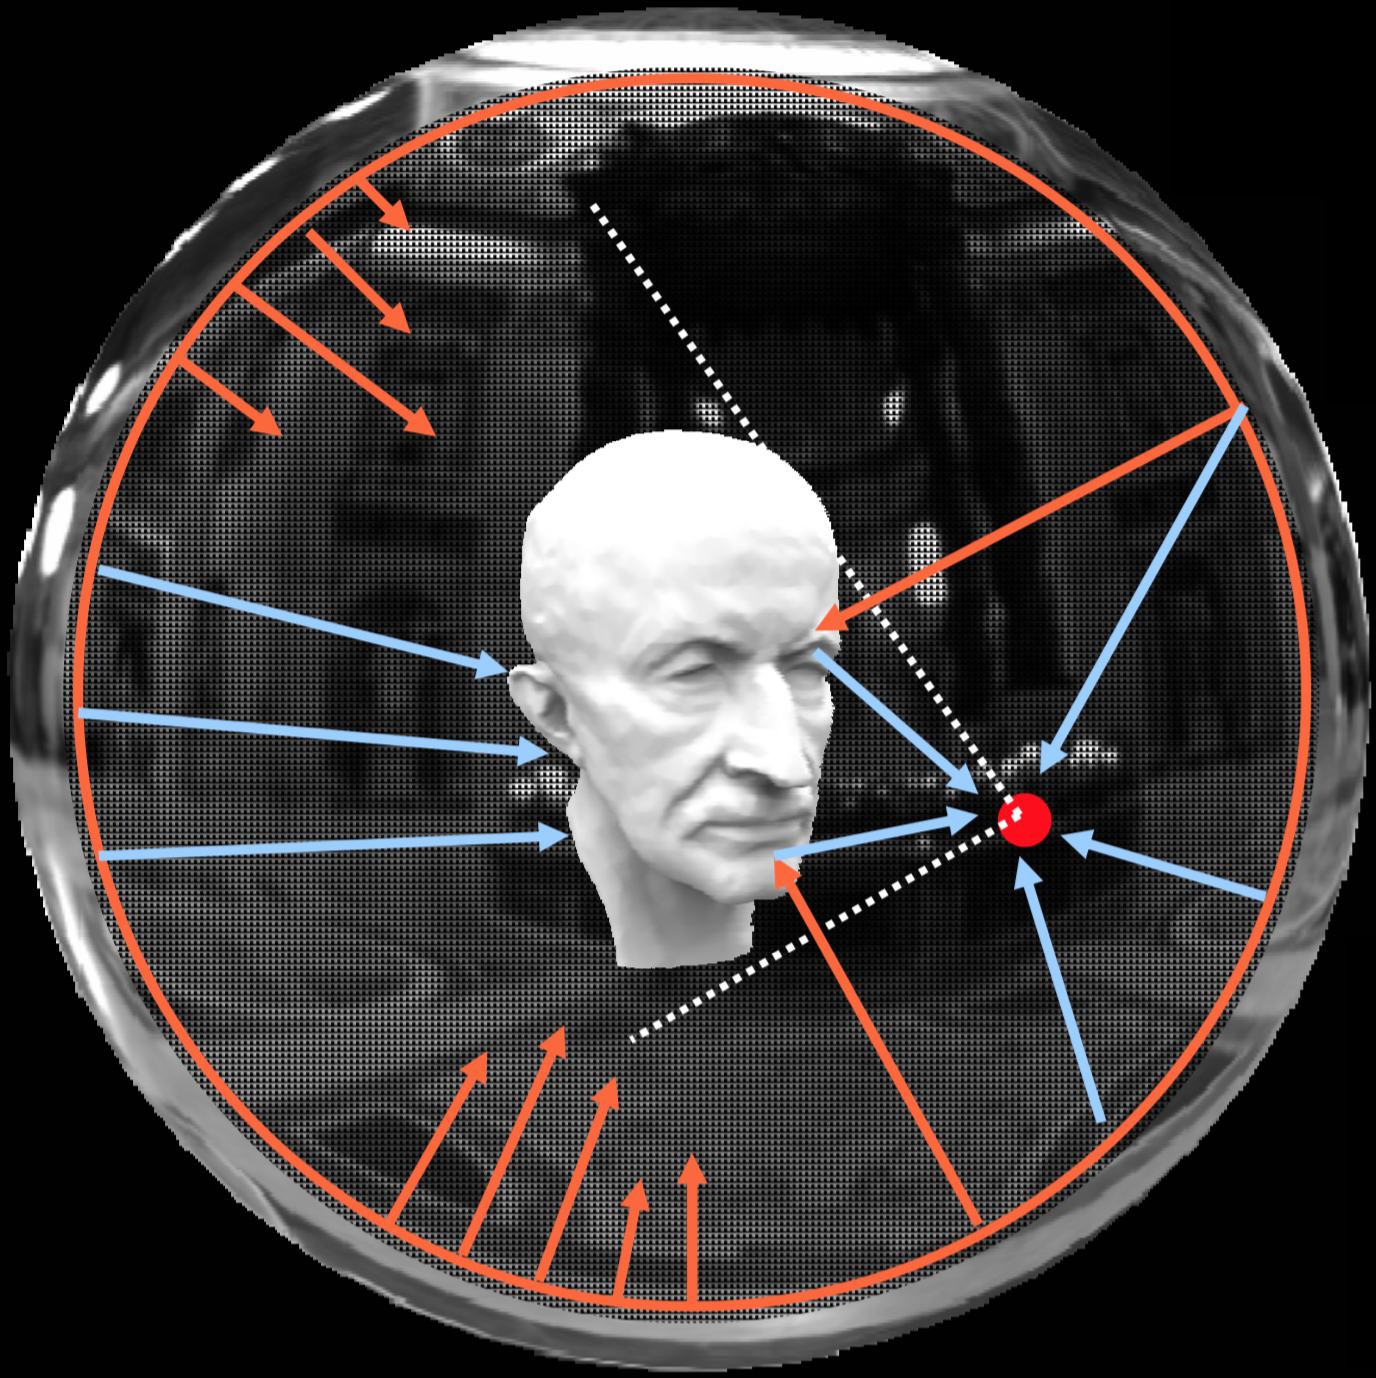
\includegraphics[width=0.65\textwidth]{graphics/prt/prt-8-2}
	\caption{What does a point $p$ near the object see?}
	\label{f:prt-goal-2}
\end{figure}

\begin{itemize}
	\item Some light proceeds directly from the lighting environment to point $p$. That happens in those directions where the object doesn't block the view from $p$.
	\item Some light that leaves the distant environment will be blocked by the object. That happens in directions where the object blocks the view from $p$ to the environment. We denote that by cutting away a part of the environment here on the right.
	\item Some light takes a bounce or multiple bounces off the object before impinging upon point $p$. In other words, $p$ sees an image of the what our object looks like when lit by the environment map.
\end{itemize}

The relationship between the lighting environment and what point $p$ sees is linear. We will in the following project the light impinging on $p$ in a finite space, and thus this relationship will be characterized by a matrix. This matrix will in general be different for each point:

\begin{equation*}
	L_{env}(\omega)\to L_{xfer}(p\leftarrow\omega)
\end{equation*}



\subsection{Transferred Incident Radiance}
In this section we will derive the exact relationship of the distant lighting environment and the lighting after it has interacted with the scene.

\begin{figure}
\sidecaption
	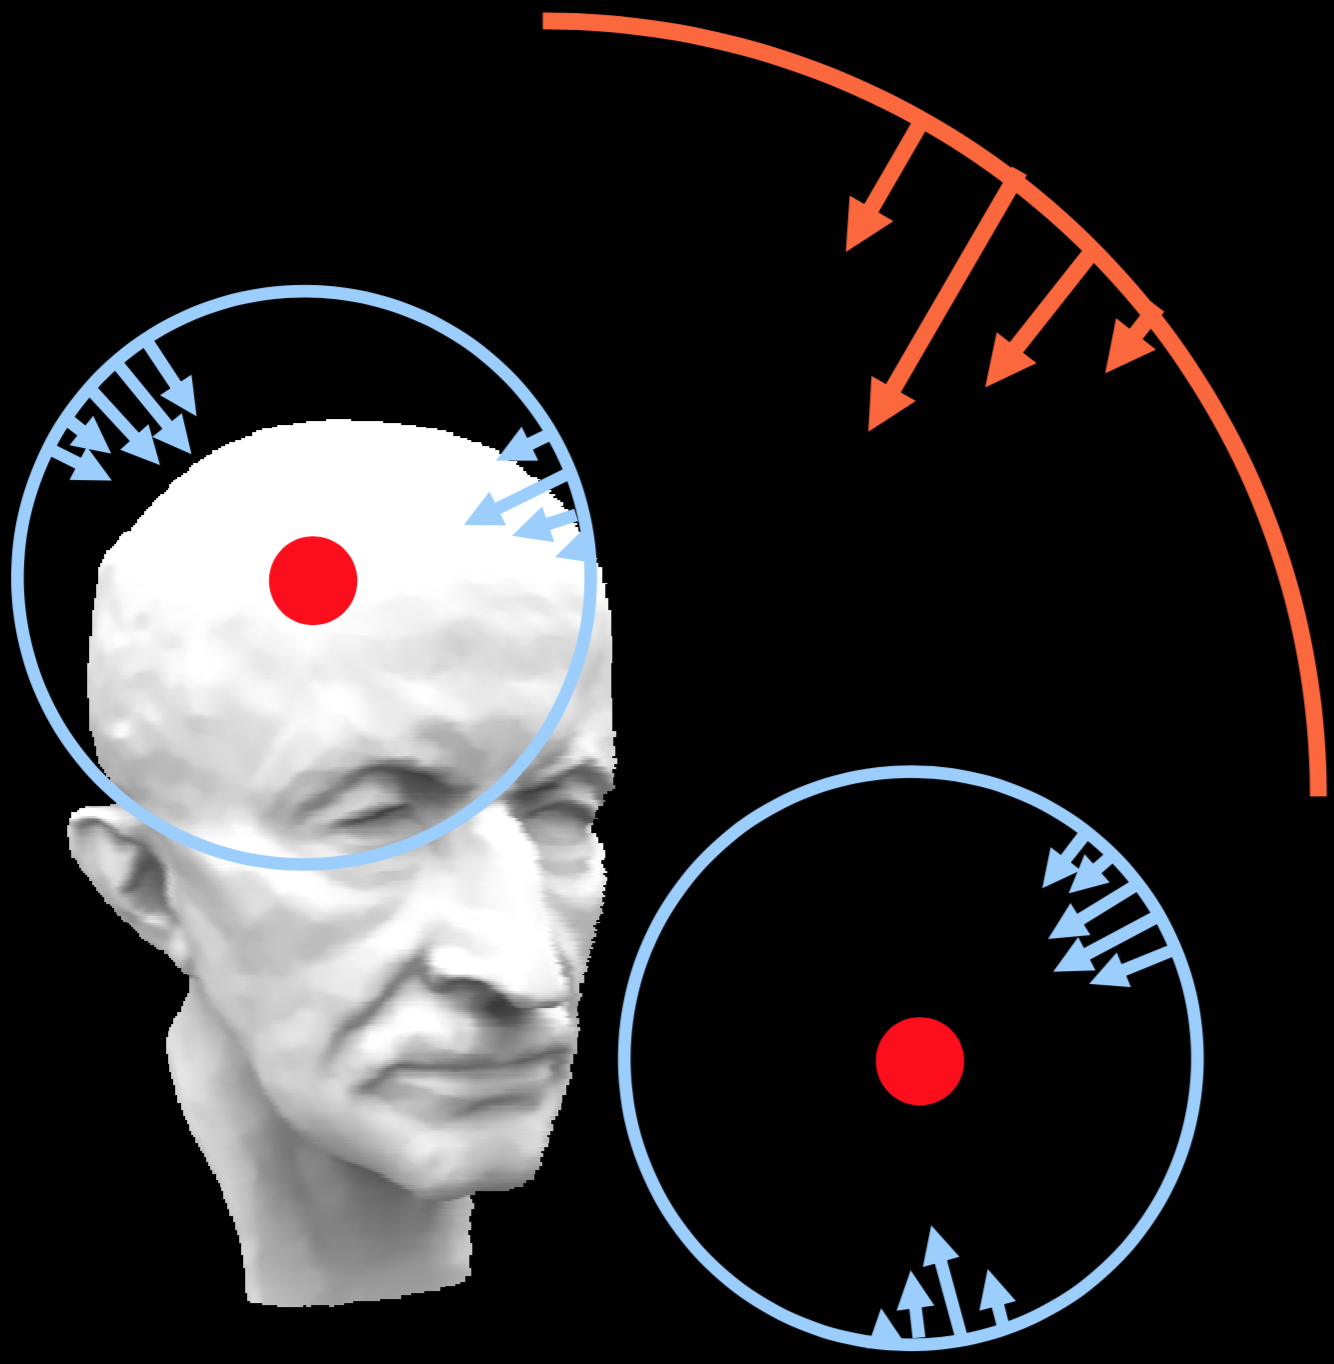
\includegraphics[width=0.65\textwidth]{graphics/prt/prt-9}
	\caption{Define transfer incident radiance $L_{xfer}(p\leftarrow\omega)$ for point $p$ as all light arriving at $p$ that originated from $L_{env}$. The point either on surface or in free space are treated unified.}
	\label{f:prt-matrix}
\end{figure}

We first define a quantity called \textit{transferred incident radiance} $L_{xfer}(p\leftarrow\omega)$, see figure \ref{f:prt-matrix}. For each point in the scene, be it on the surface of the object or in free space, we define it as the radiance incident onto that point from each direction. This is different from the distant environment, since the light is blocked and reflected by the object before impinging upon the point. In other words, it is a spherical function for each point in the scene, and it defines "what point $p$ sees", and it of course changes as the lighting environment changes.


The basic idea is that we'll precompute the linear operators (that is, matrices) that map our distant lighting environment into transferred incident radiance for discrete set of points in the scene, and at runtime we'll use them for computing transferred incident radiance at those points, given the current lighting environment.

Obviously, the light outgoing from a point on the object is the sum of emitted light and reflected light, and we get reflected light by computing the usual reflectance integral of the transferred incident lighting. This yields final reflected radiance towards the virtual camera.

So the outline of the PRT process can be seen as following:

\begin{enumerate}
	\item precompute transfer matrices off-line
	\item Use them at runtime to determine $L_{xfer}$ for surfaces to be shaded.
	\item Then integrate $L_{xfer}$ with BRDF*cosine to get outgoing radiance (just evaluate the usual reflectance equation)
\end{enumerate}

\begin{fullwidth}
\begin{tcolorbox}
So why bother with transferred incident radiance and not compute outgoing radiance directly? For surfaces of the object, this is certainly possible. But it is also possible to decouple the sampling rates of transferred incident radiance and outgoing radiance. The rationale is that transferred incident radiance often (but not always) varies quite slowly over space, whereas the outgoing radiance from a surface often has high spatial frequencies. Thus, the transferred incident radiance can often be interpolated from sparser samples, and turned into higher-frequency outgoing radiance (bi-scale radiance transfer). Of course, we want to avoid as much work as possible, and computing the transfer is expensive.
\end{tcolorbox}
\end{fullwidth}



\subsection{Derivation of Transfer Matrices}
To start the way towards deriving the transfer matrix that maps the distant illumination into transferred lighting, we project the transferred lighting into a finite, spherical function space spanned by functions $\{z\}$, see figure \ref{f:prt-tir-projection}. That is, we discretize transferred incident radiance and represent it using a finite number of basis coefficients that we denote by $l^{p}$:

\begin{figure}
\sidecaption
	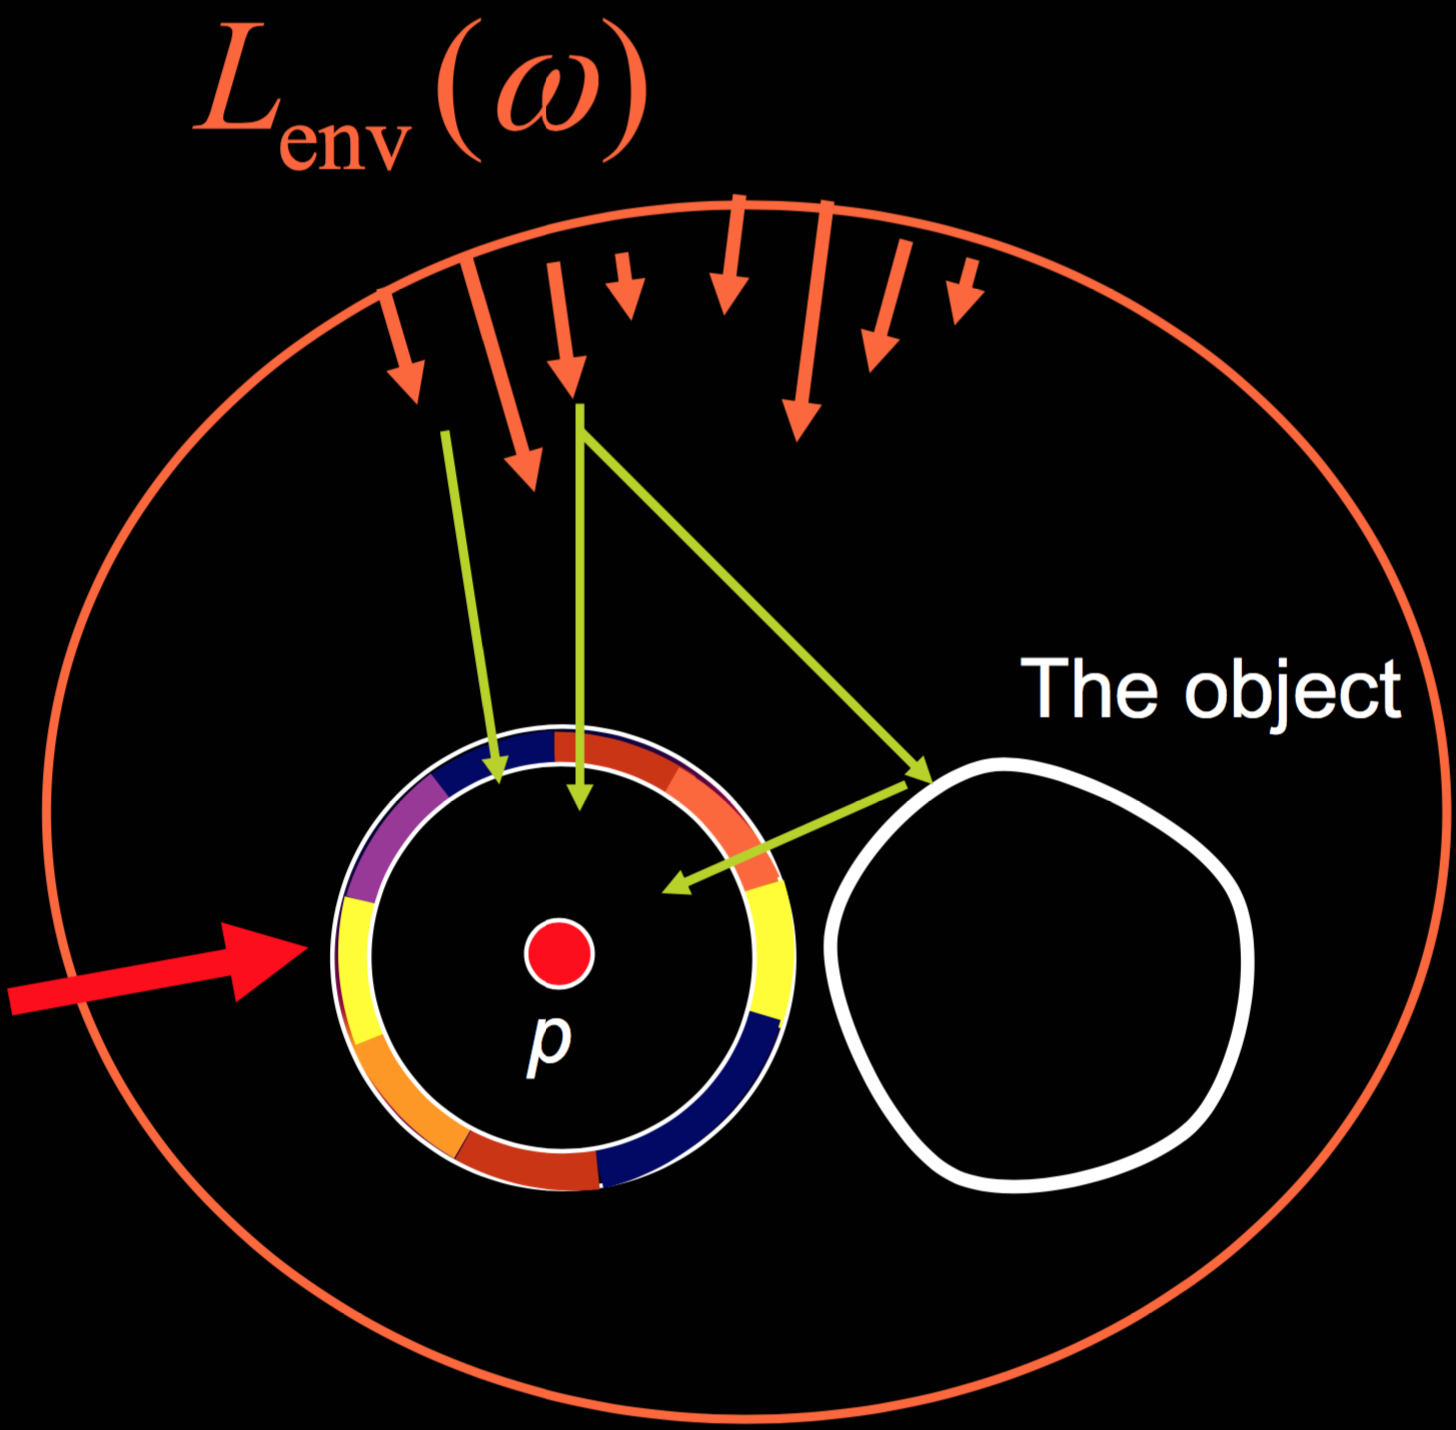
\includegraphics[width=0.65\textwidth]{graphics/prt/prt-10}
	\caption{Project transferred incident radiance at $p$ into a function space.}
	\label{f:prt-tir-projection}
\end{figure}

\begin{equation*}
	L_{xfer}(p\leftarrow\omega)\approx\sum^{m}_{i=1}l^{p}_{i}z_i(\omega)
\end{equation*}

The coefficients $l^{p}$ are unknown, the coefficients $l$ that define the distant incident lighting we know. What we want to do is find their relationship. This relationship between the two vectors is linear, and thus it can be expressed using a matrix. We call this matrix the \textit{transfer matrix} for point $p$: It maps the distant, incident illumination to an approximation of the lighting that reaches $p$:

\begin{equation*}
	l^{p}=T^{p}l
\end{equation*} 

Let's think about that for a while. What happens if the scene is lit by just a single lighting basis function $y_i$, i.e., there is just a single one in the emission vector $l$ and the rest is just zero? See figure \ref{f:prt-matrix}. That's marked there in the visual depiction as the white box in the gray vector. If we think of the matrix-vector product, in the end, it just copied the fourth column of the matrix over to the rest.

\begin{figure}
\sidecaption
	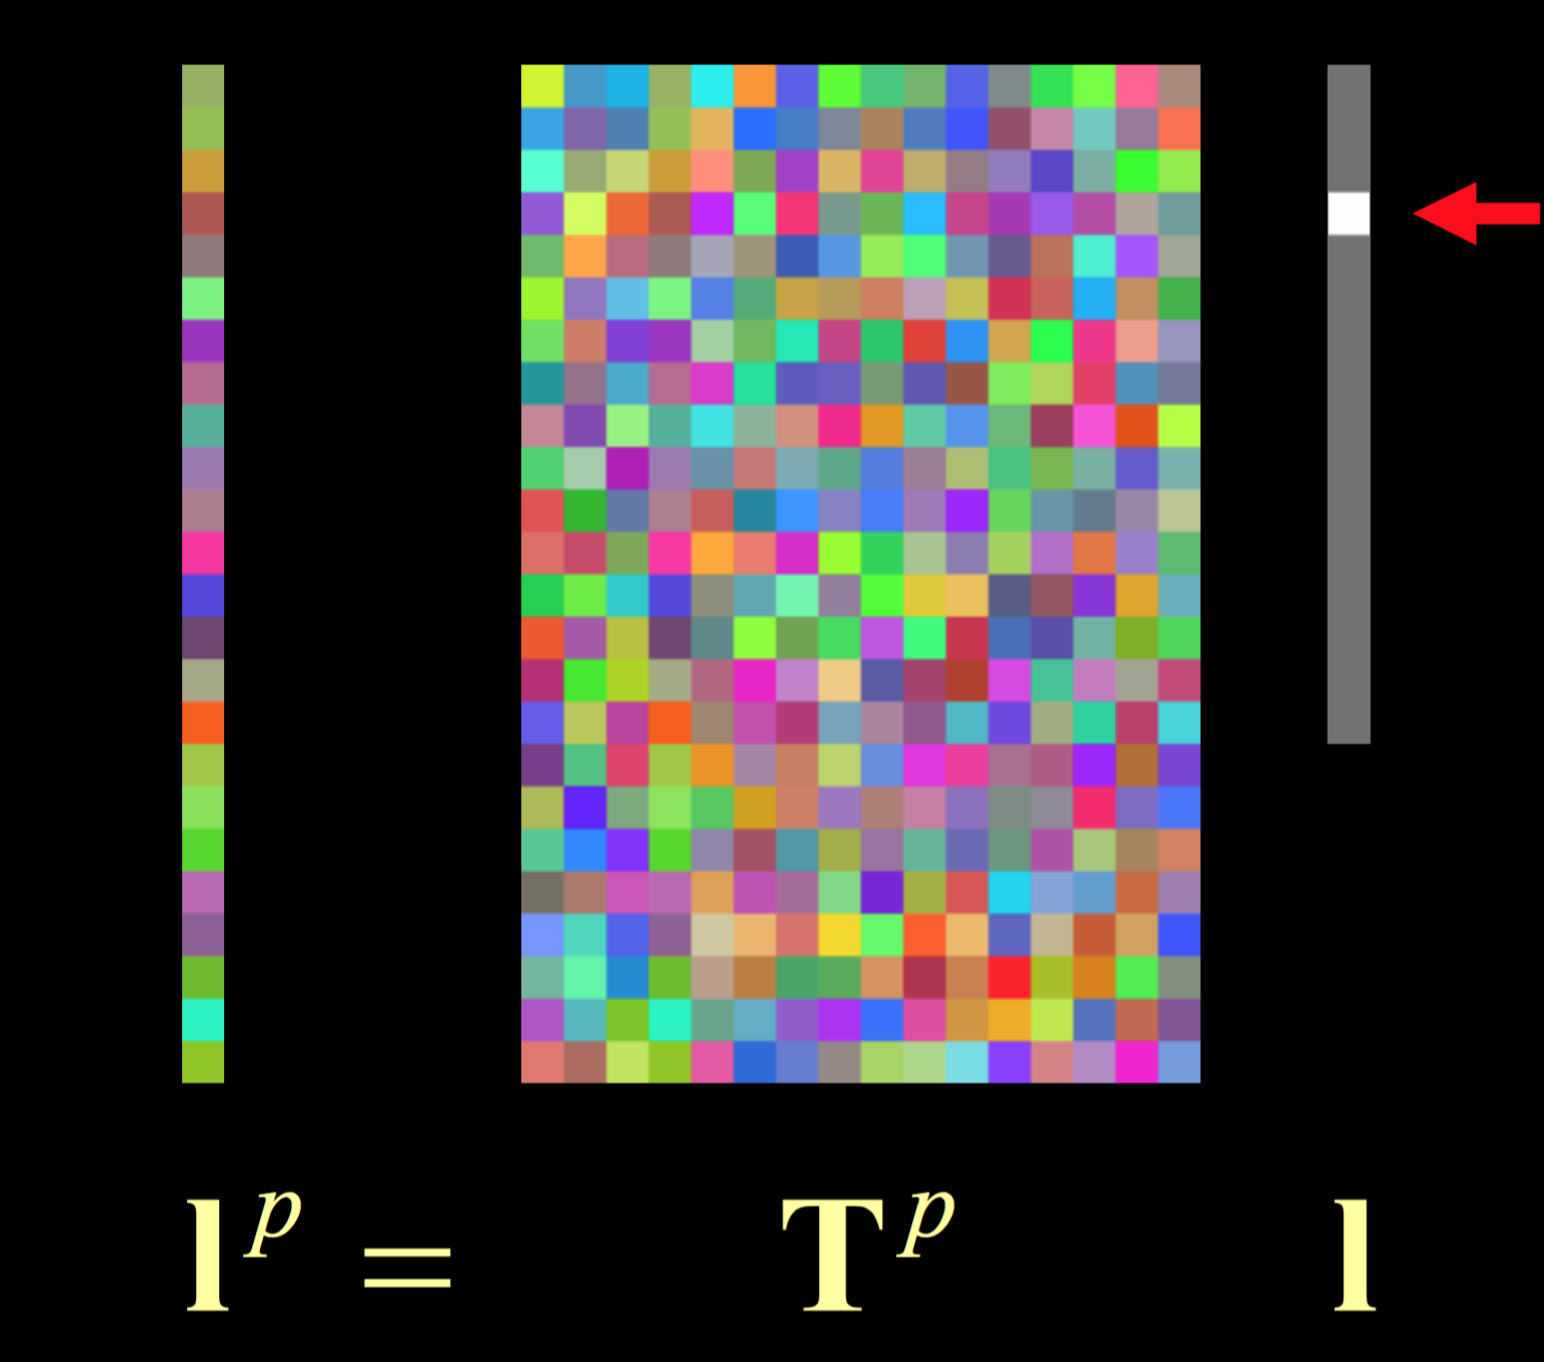
\includegraphics[width=0.65\textwidth]{graphics/prt/prt-11}
	\caption{Consider light from a single lighting basis function at unit intensity.}
	\label{f:prt-matrix}
\end{figure}

This leads us to conclude that the $i$-th column of the matrix is a \textit{basis appearance}: it describes the lighting at $p$ when the scene is lit using the $i$-th lighting basis function alone. And since the scene is lit by a linear combination of basis lights, getting the transferred incident radiance at $p$ just involves taking a linear combination of these basis appearances with weights taken from the emission vector $l$. That's just matrix-vector multiplication.




\subsection{Entries of the Transfer Matrix}
We denote that $L^{i}_{xfer}(p\leftarrow\omega)$ is the light from basis function $y_i$ that reaches $p$ either directly or through any number of bounces off the object. Then $T^{p}_{ji}$ is the $j$-th projection coefficient of $L^{i}_{xfer}(p\leftarrow\omega)$:

\begin{equation*}
	T^{p}_{ji}=\langle L^{i}_{xfer}(p),\hat{z}_j\rangle =\int_\Omega L^{i}_{xfer}(p\leftarrow\omega)\hat{z}_j(\omega)d\omega
\end{equation*}

All we need is to be able to compute the radiance that is incident to the point $p$ when the scene is lit using the $i$-th light basis function alone. These algorithms include Monte Carlo path tracing, photon mapping and progressive radiosity, etc. 

Next we'll consider the simple case of direct illumination only. That is, we consider only the light incident to the object that has been shadowed by the object, but has not bounced on the surface before impinging upon $p$. The direct lighting incident to $p$ (denote by $L_0$) is just the lighting environment modulated by the visibility from $p$:

\begin{equation*}
	L_0(p\leftarrow\omega)=L_{env}(\omega)V(p,\omega)
\end{equation*}

The direct lighting to $p$ due to basis function $y_i$ is then:

\begin{equation*}
	L^{i}_0(p\leftarrow\omega)=y_i(\omega)V(p,\omega)
\end{equation*}

and thus:

\begin{equation*}
\begin{aligned}
	T^{p}_{0,ji}=&\langle L^{i}_0(p\leftarrow\omega),\hat{z}_j\rangle \\
	=&\int_\Omega y_i(\omega)\hat{z}_j(\omega)V(p,\omega)d\omega
\end{aligned}
\end{equation*}

We call the direct-lighting-only matrix $T^{p}_0$. If we substitute the previous into the equation that gives the approximated transferred incident from the its basis coefficients, we get the following formula for the approximate lighting impinging on $p$ from the full lighting environment:

\begin{equation*}
\begin{aligned}
	L(p\leftarrow\omega)\approx &\sum^{m}_{j=1}l^{p}_{j}z_j(\omega)\\
	=&\sum^{m}_{j=1}z_j(\omega)\Biggr[ \sum^{n}_{i=1}l_iT^{p}_{ji}  \Biggr]
	=z(\omega)^{T}T^{p}l
\end{aligned}
\end{equation*} 

The sum in the middle can be written in matrix form as given on the second line, where we have stacked the values of all the basis functions $z_j$, evaluated in direction $\omega$, together to form the vector $z$.




\subsection{Accounting for Indirect Lighting}
This section derives a particular method for computing the transfer matrices that account for indirect lighting as well. It resembles a progressive gathering radiosity method, and bears a close resemblance to an early non-diffuse global illumination method.

In what follows, we'll derive a recursive formula that computes the transfer matrices that correspond to $k+1$ bounces of light, given that we know the transfer matrices that account for $k$ bounces for light everywhere in the scene. As we already have a method for computing $T_0$, the transfer matrix for direct lighting, we are able to account for an arbitrary number of bounces this way. And as lighting is linear, the transfer matrix $T^{p}$ that accounts for all bounces is just the sum of the matrices $T^{p}_0,T^{p}_1,\cdots$ that each account for a particular number of bounces.

In order to derive the method, we'll use a "transposed" version of the rendering equation. One that we have specifically using transferred incident radiance as the unknown, not outgoing radiance as is usually done. These equations are equivalent, if we know the solution to the other, we get the other pretty easily from it (see figure \ref{f:prt-transposed-version}).

\begin{figure}
\sidecaption
	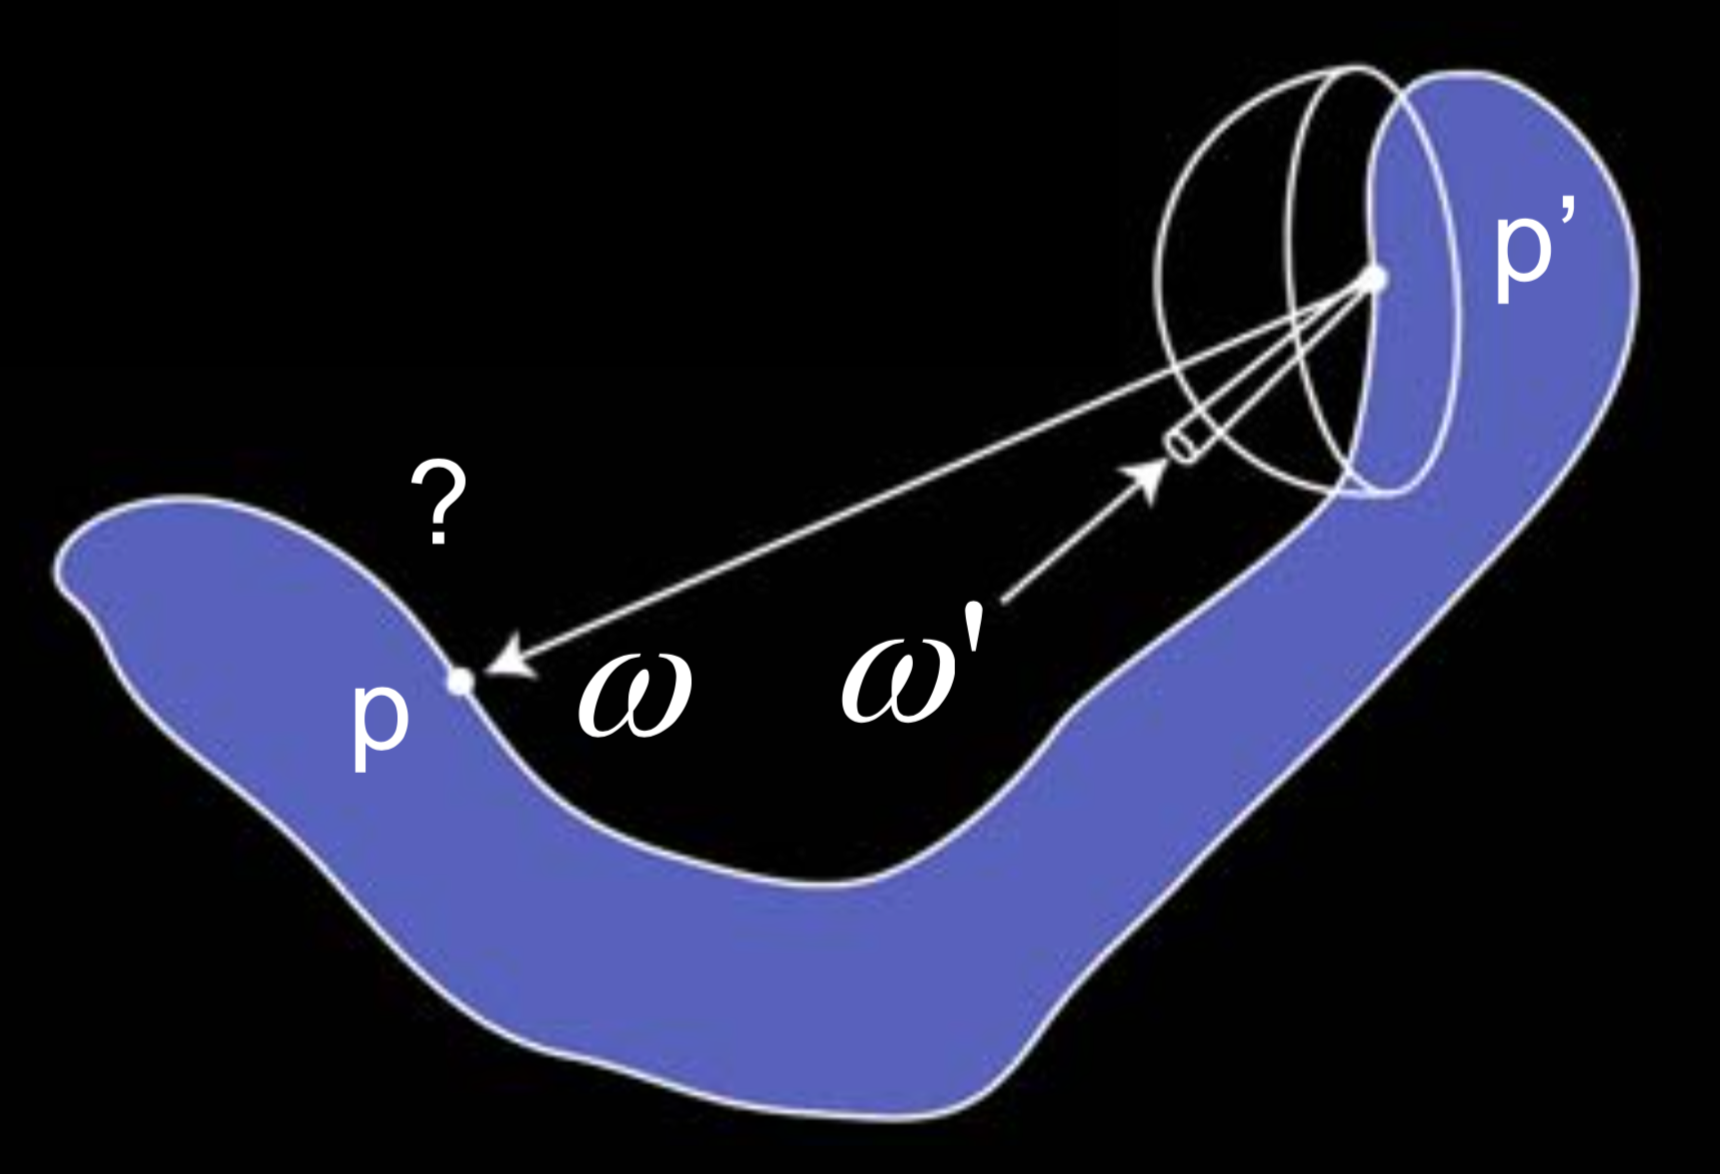
\includegraphics[width=0.65\textwidth]{graphics/prt/prt-12}
	\caption{$p^{'}$ is the point that the ray from $p$ towards $\omega$ intersects. Note that the usual reflectance integral is performed above the point $p^{'}$ here, not $p$ as in the usual version of the rendering equation.}
	\label{f:prt-transposed-version}
\end{figure}

\begin{equation*}
\begin{aligned}
	L_{xfer}(p\leftarrow\omega)=&L_{env}(\omega)V(p,\omega)\\
	&+\int_{\Omega (p^{'})}L_{xfer}(p^{'}\leftarrow\omega^{'})f_r(p^{'},\omega^{'}\to -\omega)cos\theta^{'}d\omega^{'}
\end{aligned}
\end{equation*}

This equation says that the lighting incident to $p$ is the sum of:

\begin{itemize}
	\item Direct lighting from the lighting environment, shadowed by the object.
	\item Lighting reflected by the scene towards $p$.
\end{itemize}

The incident version of the rendering equation can be solved using Neumann series just as well as the outgoing version: the lighting upon $p$ is the sum of direct light, light that has taken one, two, three, etc. bounces.

Given that we know the lighting in the scene that has taken $k$ bounces, then the Neumann series gives the relationship of this known $k$-times reflected light and $k+1$-times reflected light, i.e., if we know the incident radiance from the previous bounce, the next one is obtained from the reflectance equation:

\begin{equation*}
	L_{k+1}(p\leftarrow\omega)=\int_{\Omega (p^{'})}L_k(p^{'}\leftarrow\omega^{'})f_r(p^{'},\omega^{'}\to -\omega)cos\theta^{'}d\omega^{'}
\end{equation*}

To derive transfer matrices for all bounces, we'll start from the projection equation: we want to express $L_{xfer}$ at $p$ in terms of the basis functions $z$. In the end this will yield the transfer matrices for all bounces:

\begin{equation*}
	L_{xfer}(p\leftarrow\omega)\approx\sum^{m}_{j=1}l^{p}_jz_j(\omega)
\end{equation*}

As we saw earlier, in order to get the $j$-th projection coefficients, we have to integrate the function against the dual basis function $\tilde{z}$:

\begin{equation*}
	l_j^{p}=\int_\Omega L_{xfer}(p\leftarrow\omega)\tilde{z}_j(\omega)d\omega=:\langle L_{xfer}(p),\tilde{z}_j\rangle
\end{equation*}

By the Neumann series:

\begin{equation*}
	L_{xfer}(p\leftarrow\omega)=L_{0}(p\leftarrow\omega)+L_{1}(p\leftarrow\omega)+L_{2}(p\leftarrow\omega)+\cdots
\end{equation*}

Since the inner product is linear, the projection coefficients can be computed by projecting each bounce of light separately and adding the results together:

\begin{equation*}
	l^{p}_j=\langle L_0(p),\tilde{z}_j\rangle+\langle L_1(p),\tilde{z}_j\rangle+\langle L_2(p),\tilde{z}_j\rangle+\cdots
\end{equation*}




\subsection{Transfer Matrix for Bounce $k+1$}
So far, we've already derived per-point matrices $T^{p}_0$ that map coefficients of lighting environment to coefficients that represent direct lighting. We'll start the derivation of the matrices $T^{p}_{k+1}$ from the projection coefficients $l^{p}_k$.




In a non-scattering medium, points not on surfaces do not affect the appearance of the scene. So just compute solution with all bounces for surface points first, then gather all bounces at once for points in free space.


\subsection{Outgoing Radiance}



\section{All-Frequency PRT}

All-Frequency Relighting of Glossy Objects.pdf
Our system approaches the sampling problem by choosing a high sampling rate for the lighting but a low sampling rate for the view. This is achieved by combining non-linear wavelet approximation for the lighting with low-order separable approximation for the BRDF. As a result, we have bandlimited high-frequency specularities; however, unlike the spherical harmonics based approach, our renderings preserve intricate all-frequency shadows while remain at interactive rates.



Ng et al. [129] introduce the use of wavelets for high-frequency illumination. Wavelet coefficients are selected on-the-fly to achieve a nonlinear approximation of high quality. This system demonstrates interactive performance for fixed viewing of nondiffuse scenes and arbitrary viewing of diffuse scenes. Figure 8.19 compares spherical harmonics with wavelets.

High-frequency illumination effects, such as sharp shadows, cannot be rep- resented with great fidelity using a small number of coefficients in the spher- ical harmonics basis functions. The next major set of innovations in PRT aim at supporting both all-frequency illumination effects and generalized BRDFs.
















